% File: cambiamenti.tex
% Created: 2015-01-22
% Author: Tesser Paolo
% Email: p.tesser921@gmail.com
% 
%
% Modification History
% Version	Modifier Date	Author			Change
% ====================================================================
% 0.0.1		2015-01-22		Tesser Paolo	inserita sezione capitolo
% ====================================================================
% 0.0.2		2015-01-28		Tesser Paolo	spiegazione pack objrem + diagramma
% ====================================================================
%


\section{Cambiamenti e Aggiunte} % (fold)
\label{sec:cambiamenti_e_aggiunte}
In questa sezione verranno descritti i cambiamenti e le aggiunte apportate alla precedente versione per permettere al programma di essere distribuito tra un server e più client (come evidenziato nella sezione \ref{sec:note_introduttive}). \\
Non sono state effettuate particolare revisioni al codice sviluppato per soddisfare i requisiti della seconda parte. \\
\'E stata cancellata solo la classe \textbf{PuzzleSolver}, responsabile dell'esecuzione del programma, non più necessaria, a favore di due nuove classi: \textbf{PuzzleSolverServer} e \textbf{PuzzleSolverClient}, responsabili dell'esecuzione del programma sul server e di quello sul client. Nella sezione \ref{sec:logica_di_comunicazione_client_server} verrà illustrato quale compito svolgono attraverso il loro main queste classi.

	\subsection{Aggiunte} % (fold)
	\label{sub:aggiunte}
		\subsubsection{Package objrem} % (fold)
		\label{ssub:package_objrem}
		Questo package contiene le classi TO DO. \\
		TO DO
		\begin{figure}[htbp]
			\centering
			\centerline{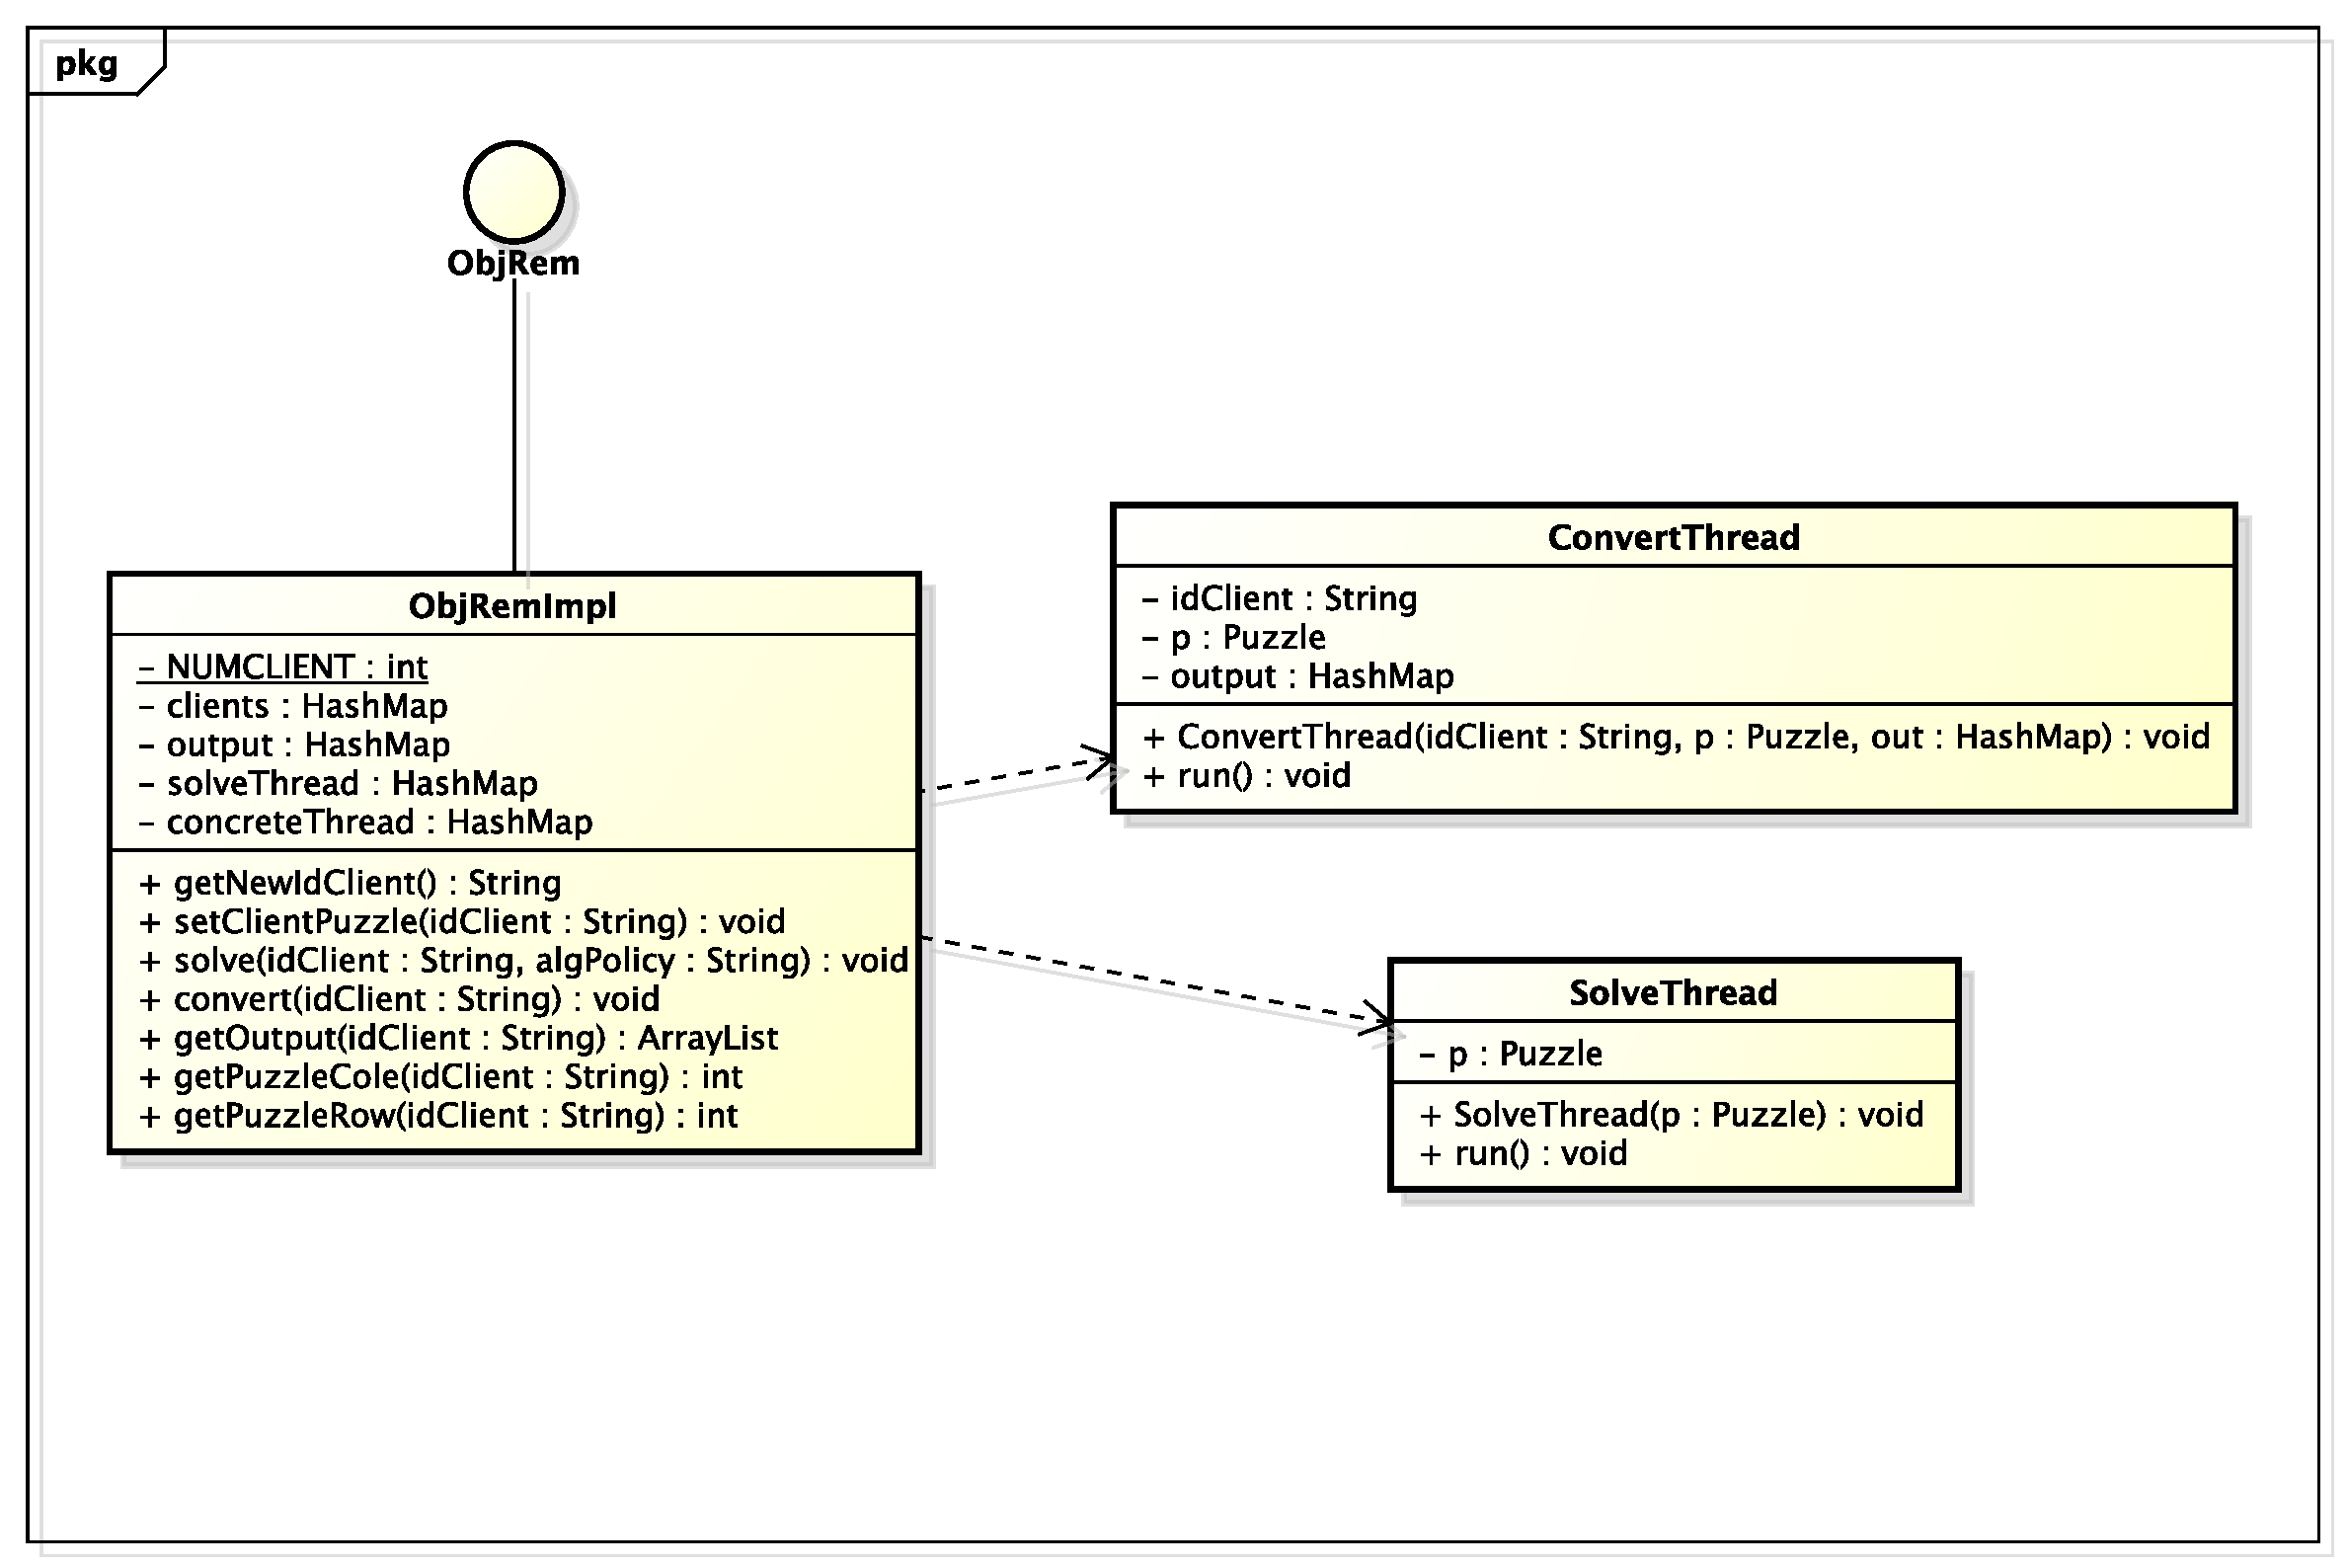
\includegraphics[scale=0.5]{img/objrem.pdf}}
			\caption{Package objrem}
			\label{Package solver}
		\end{figure}
		
		% subsubsection package_objrem (end)
	% subsection aggiunte (end)
% section cambiamenti_e_aggiunte (end)



